The Vitis Tutorials take users through the design methodology and programming model for deploying accelerated application on all Xilinx platforms.

\begin{description}
    \item [Getting Started] The basics of the Vitis programming model by putting together a very first application.
    \item [Acceleration Tutorial] Learn how to use the Vitis core development kit to build, analyze, and optimize an accelerated algorithm developed in C++, OpenCL, and even low-level hardware description languages (HDLs) like Verilog and VHDL. Learn how to use Vitis High-Level Synthesis (HLS), compiler, analyzer, and debugger to identify performance bottlenecks and make modifications to increase algorithm efficiency and performance using an Alveo Data Center acceleration card.
    \item [AI Engine Development] Learn how to use the Vitis core tools to develop for Versal, the first Adaptive Compute Acceleration Platform (ACAP) device from Xilinx. Learn how to target, develop, and deploy advance algorithms using Versal's AI Engine array in conjunction with PL IP/kernels and software applications running on the embedded processors.
    \item [Platform Creation Tutorial] Learn how to build custom platforms for Vitis to target your own boards, and how to modify and extend existing platforms. Learn how to configure the platform hardware sources, construct the runtime software environment, add support for software and hardware emulation, and more.
    \item [Vitis Developers Contributed Tutorials] Vitis-Tutorials repository for community contribution. 
    \item [Other Vitis Tutorial Repositories] Other Vitis Tutorial Repositories are as follows:
    \begin{description}
        \item [Machine Learning Tutorial] Learn how to use Vitis, Vitis AI, and the Vitis accelerated libraries to implement a fully end-to-end accelerated application using purely software-defined flows. Use Vitis AI to configure Xilinx hardware using the Tensorflow framework. Vitis AI allows the user to quantize, compile, and deploy an inference model in a matter of minutes.
        \item [Embedded Design Tutorials] Learn how to build and use embedded operating systems and drivers on Xilinx Adaptive SoCs and the MicroBlaze soft processor. These tutorials cover open-source operating systems and bare metal drivers available from Xilinx, compilers, debuggers, and profiling tools for traditional SoC software development.
    \end{description}
\end{description}

\section{Getting Started}
There are two top-level getting started tutorials for Vitis:

\begin{description}
    \item [Vitis Introduction and Getting Started] An overview of the Vitis workflow including kernel development, host software creation, emulation, implementation, and analysis, and how Vitis unifies software, acceleration, and ML development under a single development platform.
    \item [Vitis HLS] In-Depth tutorial to optimize, implement, and unit test individual hardware accelerators from within the Vitis High-Level Synthesis environment
\end{description}

\subsection{Vitis Introduction and Getting Started}
The Vitis tool provides a unified flow for developing FPGA accelerated application targeted to either Data Center accelerator cards or Embedded Processor platforms. This tutorial is divided into two separate flows: 

\begin{enumerate}
    \item Data Center flow
    \item Embedded Processor flow
\end{enumerate}

These two flows are similar in that host applications and accelerated kernels written for one flow can be used in the other flow, and the build processes are similar. However, while similar the flows are also different in that the build and runtime environments of Data Center accelerator cards and Embedded Processor platforms have different requirements that must be met.

\par This tutorial provides instructions for building and running on both the Alveo U200 Data Center accelerator card, and the Zynq Ultrascale MPSoC ZCU102 platform. These instructions can be easily adapted to other Xilinx cards.

\par The two flows in this tutorial are both organized into 5 parts and are designed to walk you through all the key aspects of the Vitis flow.

\begin{enumerate}[label=Part \arabic*:]
    \item covers all the essential concepts of the Vitis FPGA acceleration flow in under 10 minutes
    \item guides you through the process of installing the Vitis tools, platforms and runtime library.
    \item explains the source code of vector-add example used in the rest of the tutorial
    \item describes the Data Center flow and the Embedded Platform flow. Each flow includes the commands required to compile, link and run the example on your acceleration card.
    \item gives an overview of Vitis Analyzer and shows how to open and analyze reports
\end{enumerate}

\subsubsection{Part 1 : Essential Concepts}
The Vitis unified software platform provides a framework for developing and delivering FPGA accelerated applications using standard programming languages like C and C++. The Vitis flow offers all of the features of a standard software development environment, including:

\begin{itemize}
    \item  Compiler or cross-compiler for host applications running on x86 or Arm processors
    \item  Cross-compilers for building the FPGA binary
    \item  Debugging environment to help identify and resolve issues in the code
    \item  Performance profilers to identify bottlenecks and help you optimize the application
\end{itemize}
    
\paragraph{Understanding the Vitis Programming and Execution Model}
A Vitis accelerated application consists of two distinct components: a software program running on a standard processor such as an X86 processor, or ARM embedded processor, and a Xilinx device binary (xclbin) containing hardware accelerated functions, or kernels.

\par The software program, or host application, is written in C/C++ and runs on a conventional CPU. The software program uses the XRT native API implemented by the Xilinx Runtime library (XRT), or OpenCL 1.2 C/C++ API to interact with the acceleration kernel in the Xilinx device. A description of the host application and required API calls can be found in the Vitis documentation under Host Programming.

\par The hardware accelerated kernels can be written in C/C++ or RTL (Verilog or VHDL) and run within the programmable logic part of the Xilinx device. Refer to C/C++ Kernels, or RTL Kernels in the Vitis documentation for coding requirements. The kernels are integrated with a Vitis hardware platform using standard AXI interfaces.

\begin{figure}[H]
	\begin{center}
		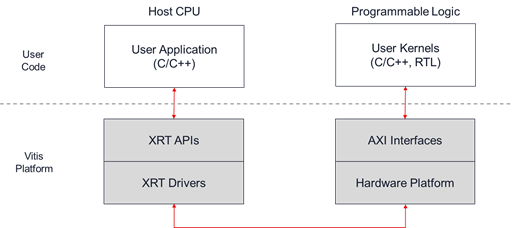
\includegraphics[width=5in]{images/part1_execution_model.png}
		\label{part1_execution_model}
	\end{center}
\end{figure}

Vitis accelerated applications can execute on either Data Center or Embedded Processor acceleration platforms:

\begin{itemize}
    \item On Data Center accelerator cards, the software program runs on an x86 server and the kernels run in the FPGA on a PCIe-attached acceleration card.
    \item On Embedded Processor platforms, the software program runs on an ARM processor of a Xilinx MPSoC device and the kernels run within the same device.
\end{itemize}

Because the software and hardware components of a Vitis application use standardized interfaces (XRT APIs and AXI protocols) to interact with each other, the user's source code remains mostly agnostic of platform-specific details and can be easily ported across different acceleration platforms.

\par There are multiple ways by which the software program can interact with the hardware kernels. The simplest method can be decomposed into the following steps:

\begin{enumerate}
    \item The host application writes the data needed by a kernel into the global memory of the FPGA device.
    \item The host program sets up the input parameters of the kernel.
    \item The host program triggers the execution of the kernel.
    \item The kernel performs the required computation, accessing global memory to read or write data, as necessary. Kernels can also use streaming connections to communicate with other kernels, passing data from one kernel to the next.
    \item The kernel notifies the host that it has completed its task.
    \item The host program transfers data from global memory back into host memory, or can give ownership of the data to another kernel.
\end{enumerate}

\paragraph{Understanding the Vitis Build Process}
The Vitis build process follows a standard compilation and linking process for both the host program and the kernel code:

\begin{itemize}
    \item  The host program is built using the GNU C++ compiler (g++) for Data Center applications or the GNU C++ Arm cross-compiler for Embedded Processor devices.

    \item The FPGA binary is built using the Vitis compiler (v++). First the kernels are compiled into a Xilinx object (.xo) file. Then, the .xo files are linked with the hardware platform to generate the Xilinx device binary (.xclbin) file. As described in Vitis Compiler Command, the Vitis compiler and linker accepts a wide range of options to tailor and optimize the results.
\end{itemize}


\begin{figure}[H]
	\begin{center}
		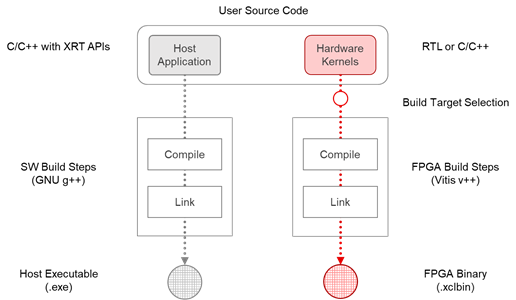
\includegraphics[width=5in]{images/part1_build_flow.png}
		\label{part1_build_flow}
	\end{center}
\end{figure}

\paragraph{Understanding Vitis Build Targets}
The Vitis compiler provides three different build targets: two emulation targets used for debug and validation purposes, and the default hardware target used to generate the actual FPGA binary:

\begin{itemize}
    \item Software Emulation - The kernel code is compiled to run on the host processor. This allows iterative algorithm refinement through fast build-and-run loops. This target is useful for identifying syntax errors, performing source-level debugging of the kernel code running together with application, and verifying the behavior of the system.
    \item Hardware Emulation - The kernel code is compiled into a hardware model (RTL), which is run in a dedicated simulator. This build-and-run loop takes longer but provides a detailed, cycle-accurate view of kernel activity. This target is useful for testing the functionality of the logic that will go in the FPGA and getting initial performance estimates.
    \item Hardware - The kernel code is compiled into a hardware description language (RTL), and then synthesized and implemented for a target Xilinx device, resulting in a binary (xclbin) file that will run on the actual FPGA.
\end{itemize}

TIP: As described in Running Emulation, there are significant differences in the build and runtime environments between Data Center and Embedded Processor platforms. These two flows will be discussed in detail in the following sections.

\subsection{Vitis HLS}

Vitis HLS Analysis and Optimization
Introduction

Vitis High-Level Synthesis (HLS) is a key part of the Vitis application acceleration development flow. The tool is responsible for compiling C/C++ and OpenCL code into a kernel for acceleration in the programmable logic (PL) region of Xilinx devices. Thus, it is the tool that compiles the hardware kernels for the Vitis tools by performing high-level synthesis.

TIP: Vitis HLS can also be used to generate Vivado IP from C/C++ code, but that flow is not the subject of this tutorial. Although similar, there are some significant differences between producing Vitis XO kernels and Vivado RTL IP. However, you can use this tutorial as a general introduction to the Vitis HLS tool.

In this tutorial, you will work through the Vitis HLS tool GUI to build, analyze, and optimize a hardware kernel. You are working through the Vitis kernel flow in the Vitis tool. For more information, refer to Enabling the Vitis Kernel Flow in the Vitis HLS Flow of the Vitis Unified Software Platform Documentation (UG1416).

Complete the labs in the following order:

\begin{itemize}
    \item Creating a Vitis HLS Project
    \item Running High-Level Synthesis and Analyzing Results
    \item Using Optimization Techniques
    \item Reviewing the DATAFLOW Optimization
\end{itemize}


\section{Acceleration Tutorial}
\section{AI Engine Development}
\section{Platform Creation Tutorial}
\section{Vitis Developers Contributed Tutorials}
\section{Other Vitis Tutorial Repositories}

\subsection{Machine Learning Tutorial}
\subsection{Embedded Design Tutorials}
